\documentclass{amsart}
\usepackage[T1]{fontenc}
\usepackage[utf8]{inputenc}
\usepackage{algorithm2e}
\usepackage{amsmath}
\usepackage{amsfonts}
\usepackage{amssymb}
\usepackage[left=2cm,right=2cm,top=3cm,bottom=3cm]{geometry}
\usepackage{graphicx}
\usepackage{hyperref}
\usepackage{dsfont}
\usepackage{cleveref}
\usepackage{bm}
\usepackage[colorinlistoftodos,bordercolor=orange,backgroundcolor=orange!20,linecolor=orange,textsize=scriptsize]{todonotes}
\definecolor{red}{cmyk}{0,1,.8,0}
\definecolor{blue}{rgb}{0,0,1}

\usepackage{xcolor}
\hypersetup{
    colorlinks,
    linkcolor={red!50!black},
    citecolor={blue!50!black},
    urlcolor={blue!80!black}
}

\usepackage{subcaption}
\SetAlgoNlRelativeSize{-1}

\ifdefined\theorem\else \newtheorem{theorem}{Theorem}\fi
\ifdefined\proposition\else \newtheorem{proposition}[theorem]{Proposition}\fi
\ifdefined\definition\else \newtheorem{definition}[theorem]{Definition}\fi
\ifdefined\lemma\else \newtheorem{lemma}[theorem]{Lemma}\fi
\ifdefined\corollary\else \newtheorem{corollary}[theorem]{Corollary}\fi
\ifdefined\remark\else \newtheorem{remark}[theorem]{Remark}\fi
\ifdefined\assumption\else \newtheorem{assumption}{Assumption}\fi
\ifdefined\example\else \newtheorem{example}{Example}\fi

\newcommand{\argmin}{\mathop{\arg\min}}

\newcommand{\nb}[3]{
		{\colorbox{#2}{\bfseries\sffamily\tiny\textcolor{white}{#1}}}
		{\textcolor{#2}{\text{$\blacktriangleright$}{\textcolor{#2}{#3}}\text{$\blacktriangleleft$}}}}
\newcommand{\rp}[1]{\nb{RP}{red}{#1}}
\newcommand{\af}[1]{\nb{AF}{blue}{#1}}
\newcommand{\bt}[1]{\nb{BT}{orange}{#1}}
\newcommand{\RR}{\mathbb{R}}

\title{Scenario reduction}

\begin{document}
\LinesNumbered
\RestyleAlgo{boxruled}
\maketitle
In this draft, I'm writting a summary of \cite{rujeerapaiboon_scenario_2022} to gather important elements of finite scenario reduction . Various proofs can get very technical and will be skipped for brevity. I'll also explore new ways of considering this problem.

\section{Introduction}
\subsection{Why ?}
From a finite distribution, the aim of scenario reduction is to compute a distribution that is close to the initial one but with a reduced number of atoms. Why would that be useful ? Take a stochastic program that can be written as : 
$$
\min_{x\in X}\int_\Xi f\left(x,\xi\right)P\left(d\xi\right)
$$
To compute a solution of this program, one uses numerical integral techniques which modify the objective function such as :
$$
\min_{x\in X}\sum_{i\in I} f\left(x,\xi_i\right)p_i
$$
with $p_i=P\left(\{\xi_i\}\right)$. The function $f$ can be expensive to compute, then a good idea would be to reduce the number of atoms of $P$ without throwing away its structure.
\subsection{Context}
In this part, we present tools and concepts useful for scenario reduction. We will define distance between two distributions : the Wasserstein distance is a good candidate. In the case of discrete distributions $\mathbb{P}=\sum_{i\in I}p_i\delta_{x_i}$ and $\mathbb{Q}=\sum_{j\in J}q_j\delta_{y_j}$, one can note that $x_i$ and $y_j$ must live in the same normed space ($\lVert\cdot\rVert$ denotes the norm). The type-$l$ Wasserstein distance between $\mathbb{P}$ and $\mathbb{Q}$ is defined as :  
\[
d_l(\mathbb{P},\mathbb{Q})=\left(\min_{\pi\in\mathbb{R}_+^{\lvert I\rvert\times\lvert J\rvert}}\left\{ 
\sum_{i\in I}\sum_{j\in J}\pi_{ij}\lVert x_i-y_j\rVert^l \: \text{ : } \:  \begin{aligned}
& \sum_{j\in J}\pi_{ij}=p_i \: \forall i\in I \\
& \sum_{i\in I}\pi_{ij}=q_j \: \forall j\in J
\end{aligned}\right\}\right)^{1/l}.
\]
The parameter $l$ has to be greater than or equal to 1 in order to satisfy axioms of distances, see \Cref{distance}. One can \bt{To prove that $d^\ell$ is distance, the difficult part is the triangle inequality. It is a distance for $\ell \geq 1$ and the proof of the triangle inequality is here called the "gluing lemma" (Peyré-Cuturi chapter 1 for our "simple" case). This gluing lemma uses Minkowski's inequality in the case $\ell\geq1$ so that's the reason why. 
It is still an interesting question for $0 < \ell \leq 1$. We have $d_\ell^\ell$ (and not $d\ell$ itself) is a distance as $(x,y) \mapsto \lVert x - y \rVert^\ell$ is already a distance when $0 < \ell \leq 1$ thanks to Minkowski's inequality in the case $\ell \leq 1$.
}. See \Cref{compute} in order to have an idea on how to compute the distance of Wasserstein between two distributions and more precision.
\newline

$\mathcal{P}_E(X,n)$ denotes the set of all \textbf{uniform} discrete distribution on $X\subset R^d$ with \textbf{exactly} $n$ distinct scenarii and $\mathcal{P}(X,m)$ denotes the set of discrete distributions on $X\subset R^d$ with \textbf{at most} m scenarii. In the article, one assume that $\mathbf{P}\in\mathcal{P}_E(X,n)$. What is true when you obtain the distribution $\mathbb{P}$ via sampling, every issue has the probability of $\frac{1}{n}$ and if a same value occurs twice or more, they say we can decompose the distribution with two or more close atoms.
\newline

We want to find a distribution that minimizes the Wasserstein distance over a particular set of distribution just like we can do in $\RR^d$ when we want to project a point over a subspace. Two types of reduction are typically presented. The continous scenario reduction problem :
$$
C_l(\mathbb{P},m)=\min_\mathbb{Q}\left\{d_l(\mathbb{P},\mathbb{Q}),\: \mathbb{Q}\in\mathcal{P}(\mathbb{R}^d,m)\right\}. 
$$
The discrete scenario reduction problem :
$$
D_l(\mathbb{P},m)=\min_\mathbb{Q}\left\{d_l(\mathbb{P},\mathbb{Q}),\: \mathbb{Q}\in\mathcal{P}(\text{supp}(\mathbb{P}),m)\right\}.
$$
Let $\mathbb{P}$ be a finite distribution on $\RR^d$, obviously $\text{supp}(\mathbb{P})\subset \mathbb{R}^d$ leads to $C_l(\mathbb{P},m)\leq D_l(\mathbb{P},m)$. Discrete scenario reduction problem has been more studied as it uses atoms of $\mathbb{P}$ that have a physical reality (if $\mathbb{P}$ represents the distribution of a real event).

\section{Fundamental limits of scenario reduction}\label{limit}
\subsection{Bounds}
Here, we try to provide bounds on the value of the Wasserstein distance in order to guarantee closeness between the reduced distribution and the original one. We work with $\lVert\cdot\rVert_2$ and atoms within the unit ball because of the positive homogeneity of the Wasserstein distance $C_l(\mathbb{P}^\lambda,m)=\lambda \cdot C_l(\mathbb{P},m)$ for $\lambda\in\mathbb{R}_+$ and $\mathbb{P}^\lambda=\sum_{i\in I}p_i\delta_{\lambda\cdot x_i}$. See \Cref{scaled} for a proof. \rp{not obvious tbh} Generally, we have that : $$\forall \lambda\in\mathbb{R}, C_l(\mathbb{P}^\lambda,m)=|\lambda|C_l(\mathbb{P},m).$$ 
The homogeneity allows us to investigate inside the unit ball as we can scale distributions w.l.o.g. Another goal of this part is to quantify and study the worst case of scenario reduction defined by :
$$
\bar{C}_l\left(n,m \right)=\left\{\max_{\mathbb{P}\in\mathcal{P}_E(\mathbb{R}^d,n)}C_l(\mathbb{P},m)\: :\: \text{supp}(\mathbb{P})\in B(0,1)\right\}.
$$
The goal is to find an upper bound better than 1 for $\bar{C}_l\left(n,m \right)$. First, we prove that : $\bar{C}_l\left(n,m \right)\leq 1$. By definition, for $\mathbb{P}\in\mathcal{P}_E(\mathbb{R}^d,n)$, we have that : 
$$d_l(\mathbb{P},\delta_0)^l=\left(\min_{\pi\in\mathbb{R_+^n}}\left\{ 
\sum_{i=1}^n\pi_i\lVert x_i\rVert^l \: \text{ : } \:  \begin{aligned}
& \pi_{i}=p_i, \: \forall i\in I \\
& \sum_{i= 1}^n\pi_{i}=1 
\end{aligned}\right\}\right)\leq\left(\min_{\pi\in\mathbb{R_+^n}}\left\{ 
\sum_{i=1}^n\pi_i \: \text{ : } \:  \begin{aligned}
& \pi_{i}=p_i, \: \forall i\in I \\
& \sum_{i= 1}^n\pi_{i}=1 
\end{aligned}\right\}\right)=1.$$
Here we used that $\lVert x_i\rVert\leq 1$ and positivity of $\pi$. Again by definition, we have that
$$
C_l(\mathbb{P},m)\leq C_l(\mathbb{P},1)\leq d_l(\mathbb{P},\delta_0)\leq 1.
$$
The right hand side which is 1 doesn't depend on $\mathbb{P}$, so we can go to the upper bound for $\mathbb{P}\in\mathcal{P}_E(\mathbb{R}^d,n), \text{supp}(\mathbb{P})\in B(0,1)$ and we proved that $\bar{C}_l\left(n,m \right)\leq1$ \rp{this bound even works for non uniform discrete distributions and doesn't matter on the norm we use as long as $\text{supp}(\mathbb{P})\in B(0,1)$ for the norm}
The aim of what's next is to tighten that bound for $l\in\{0,1\}$ and with $\lVert\cdot\rVert_2$.
\newline

$\mathfrak{P}(I,m)$ is the family of m-set partitions of $I$. Following \cite{rujeerapaiboon_scenario_2022}, we write $\{I_j\}$ an element of $\mathfrak{P}(I,m)$ and $I_j$ for $j\in\{1,..,m\}$ a set of the partition $\{I_j\}$.
\begin{theorem}{Reformulation}\label{theorem1}
$$C_l(\mathbb{P},m)=\min_{\{I_j\}\in \mathfrak{P}(I,m)}\left\{ \frac{1}{n}\sum_{j\in J}\min_{y_j\in\mathbb{R}^d}\sum_{i\in I_j}\lVert x_i-y_j\rVert^l \right\}^{1/l}.$$
\end{theorem}

\begin{remark}
    For $l=2$, the inner minimum, $y_j^*=\frac{1}{|I_j|}\sum_{i\in I_j}x_i$. For $l=1$, $y_j^*$ is attained by any geometric median (minimizer of the distance - not squared - to a family). Indeed, let $\{I_j\}\in\mathfrak{P}\left(I,m\right)$ and $I_j\in\{I_j\}$ fixed. We want to compute the inner minimum : 
    $$
    \min_{y\in\RR^d}f(y)=\min_{y\in\RR^d}\sum_{i\in I_j}\lVert x_i-y\rVert^2.
    $$
    We have to minimize an unconstrained function, when we work with $\lVert\cdot\rVert_2$, the gradient of $f$ is : 
    $$
    \nabla f(y)=-2\sum_{i\in I_j}\left(x_i-y\right).
    $$
    This gradient is worth $0_{\RR^d}$ when :
    $$
    y=\frac{1}{n}\sum_{i\in I_j}x_i=\text{mean}\left(I_j\right).
    $$
    The Hessian is :    $$\nabla^2f\left(\text{mean}\left(I_j\right)\right)=2Id_d\succcurlyeq 0$$
\end{remark}

\begin{theorem} Type-2 Wasserstein distance upper bound
    $$\bar{C}_2\left(n,m \right)\leq \sqrt{\frac{n-m}{n-1}}.$$
\end{theorem}
\begin{proof}
    We give a sketch of the proof. From \Cref{theorem1} and its remark, we have that : 
    \begin{align*}\bar{C}_2\left(n,m\right)=&
        \max_{\{y_i\}\subseteq\RR^d}\min_{\{I_j\}\in\mathfrak{P}\left(I,m\right)}\left[\frac{1}{n}\sum_{j\in J}\sum_{i\in I_j}\lVert y_i-\text{mean}\left(I_j\right)\rVert_2^2\right]^{1/2} \\ &\lVert y_i\rVert_2\leq1 \:\forall i\in I
    \end{align*}
    Now, they reformulate this as : 
    \begin{align*}\bar{C}_2\left(n,m\right)^2=&
        \max_{\tau\in\RR, \{y_i\}\subseteq\RR^d}\quad\frac{1}{n}\tau \\ &\text{s.t. }\tau\leq\sum_{j\in J}\sum_{i\in I_j}\lVert y_i-\text{mean}\left(I_j\right)\rVert_2^2\; :\; \forall \{I_j\}\in\mathfrak{P}\left(I,m\right) \\
        &\quad\quad y_i^Ty_i\leq1 \quad\quad\quad\quad\quad\quad\quad\quad\quad : \forall i\in I
    \end{align*}
    The use of $\tau$ is legit as the first constraint means that $\tau\leq\min_{\{I_j\}}\sum_{j\in J}\sum_{i\in I_j}\lVert x_i-\text{mean}(I_j)\rVert_2^2$ but as we want to maximize the function $\tau$ will be the highest he can, so it'll be equal to the minimum, thereafter it gets technical but understandable. To your best understanding of the proof in \cite[Theorem 2]{rujeerapaiboon_scenario_2022} two lemmas are used to prove this inequality. Lemma 1 is kind of technical as the set of solutions of a convex problem is convex, which is necessary to say that : $S=\frac{1}{n!}\sum_{\sigma\in\mathfrak{S}}S^\sigma$ is also a solution. This matrix S is indeed invariant under permutations. Lemma 2 is easy but I give an easier proof in \Cref{eigen}.
\end{proof}

Then the article highlights a distribution \textbf{that reaches the upper bound for \boldmath{$d\geq n-1$}(meaning that the upper bound is optimal)} under these assumptions. We now treat the case $l=1$.

\begin{theorem}
    $$\bar{C}_1\left(n,m \right)\leq\bar{C}_2\left(n,m \right) \leq\sqrt{\frac{n-m}{n-1}}.$$
\end{theorem}

\begin{proof}
    \begin{align*}\bar{C}_1\left(n,m\right)=&
        \max_{\{y_i\}\subseteq\RR^d}\min_{\{I_j\}\in\mathfrak{P}\left(I,m\right)}\frac{1}{n}\sum_{j\in J}\sum_{i\in I_j}\lVert y_i-\text{gmed}\left(I_j\right)\rVert_2 \\ &\lVert y_i\rVert_2\leq1 \:\forall i\in I
    \end{align*}
    By definition of the geometric median we have that : $$\sum_{i\in I_j}\lVert x_i-\text{gmed}(I_j)\rVert_2\leq \sum_{i\in I_j}\lVert x_i-\text{mean}(I_j)\rVert_2, \: \forall j\in J.$$ 
    Then we have that :
    \begin{align*}
        \bar{C}_1\left(n,m\right)&\leq
        \max_{\{y_i\}\subseteq\RR^d}\left\{\min_{\{I_j\}\in\mathfrak{P}\left(I,m\right)}\frac{1}{n}\sum_{j\in J}\sum_{i\in I_j}\lVert y_i-\text{mean}\left(I_j\right)\rVert_2\quad,\quad \lVert y_i\rVert_2\leq1 \:\forall i\in I  \right\}\\ 
        &\leq\max_{\{y_i\}\subseteq\RR^d}\left\{\min_{\{I_j\}\in\mathfrak{P}\left(I,m\right)}\left[\frac{1}{n}\sum_{j\in J}\sum_{i\in I_j}\lVert y_i-\text{mean}\left(I_j\right)\rVert_2^2\right]^{1/2}, \quad\lVert y_i\rVert_2\leq1 \:\forall i\in I\right\} \\
        &=\bar{C}_2\left(n,m\right).
    \end{align*}
    Where the last inequality comes from Cauchy-Schwartz inequality. For all $i\in[\![1;n]\!], x_i\in\RR^d$, 
    $$
    \frac{1}{n}<x,\mathbf{1}>=\frac{1}{n}\sum_{i=1}^nx_i \leq \frac{\sqrt{n}}{n}\lVert x\rVert=\sqrt{\frac{\sum_{i=1}^nx_i^2}{n}}.
    $$
    In that case, $d=1, x_{ij}\gets y_i-\text{mean}\left(I_j\right)$.
\end{proof}
Maybe the bound can be tightened because the proof only proves : $$\bar{C}_1\left(n,m \right)\leq\bar{C}_2\left(n,m \right).$$
Unlike $\bar{C}_2\left(n,m \right)$, we also get a lower bound on $\bar{C}_1\left(n,m \right)$: $$\bar{C}_1\left(n,m \right)\geq\sqrt{\frac{(n-m)(n-m+1)}{n(n-1)}}\geq \frac{n-m}{n-1}.$$
Now the right hand side equals $\bar{C}_2^2(n,m)$ whenever $d\geq n-1$. Then we can write the following proposition :
\begin{proposition}Whenever $d\geq n-1$,  
$$\bar{C}_2^2\left(n,m \right)\leq \bar{C}_1\left(n,m \right)\leq\bar{C}_2\left(n,m \right).$$
\end{proposition}
\subsection{Use of bounds}
One can use the bounds we found above in order to guarantee that the reduced distribution is close enough (to be defined...) to the original one. For $l\in\{1,2\}$ and a large $n$ : $$\bar{C}_l\left(n,m \right)\leq \sqrt{\frac{n-m}{n-1}}=\sqrt{\frac{1-\frac{m}{n}}{1-\frac{1}{n}}}\underset{n \to +\infty}{=}\sqrt{1-\frac{m}{n}}(1+\frac{1}{2n}+O(\frac{1}{n^2}))\approx \sqrt{1-\frac{m}{n}}.$$
This latest result and the positive homogeneity of $C_l$ provides an upper bound that depends only on the ratio $p=\frac{m}{n}$ for all kind of discrete distribution $\mathbb{P}=\frac{1}{n}\sum_{i\in I}\delta_{x_i}$. Denote by $r\geq 0$ and $\mu\in\mathbb{R}^d$ the radius and the center of any  (ideally the smallest) ball enclosing $\text{supp}(\mathbb{P})$, we have that :
$$
C_l(\mathbb{P},m)=r\cdot C_l(\frac{1}{n}\sum_{i\in I}\delta_{\frac{x_i-\mu}{r}},m)\leq r\cdot \bar{C_l\left(n,m \right)}\leq r\cdot \sqrt{1-p}.
$$
One can think that $C_l(\mathbb{P},m)$ is much smaller than $r\cdot \sqrt{1-p}$ but in fact it often happens even when $\left\{x_i\right\}$ are sampled from a normal distribution for example, see \textbf{Proposition 3} of \cite{rujeerapaiboon_scenario_2022}.
As an example, we can choose : $\mu=\frac{1}{n}\sum_{i\in I}x_i$ and $r=\max_i\left\{{\lVert x_i-\mu\rVert}\right\}$. One can easily verify that this couple defines a ball enclosing $\text{supp}\left(\mathbb{P}\right)$. Then it follows that : 
$$
C_l(\mathbb{P},m)\leq \max_i\left\{{\lVert x_i-\mu\rVert}\right\}\sqrt{1-p}.
$$
what depends only on $\mathbb{P}$. \rp{maybe that helps a very little the article}. A good idea \rp{imo} is to find the smallest bound for a given distribution $\mathbb{P}$ and a given norm $\lVert\cdot\rVert$, so we can have a better upper bound. One must find the Chebyshev center (see \Cref{chebyshev}) :
\begin{align*}
    &\min_{r\in\RR^+,\mu\in\RR^d} \quad r\\
    &\text{s.t.}\quad \lVert\frac{x_i-\mu}{r}\rVert \leq 1, \;\forall i\in I.
\end{align*}
\newline

\section{What about discrete scenario reduction}
Naturally, the continuous scenario reduction gives a smaller distance than the one computed by the discrete scenario reduction. We'll try to quantify and compare the gap between the solution of both problems. More precisely, in this part, we find for $l\in\{1,2\}$: 
$$\underline{\kappa}_l\left(n,m\right)\cdot C_l\left( \mathbb{P},m\right)\leq D_l\left(\mathbb{P},m\right)\leq \bar{\kappa}_l\left(n,m\right)\cdot C_l\left(\mathbb{P},m\right)$$
The goal is to find the largest $\underline{\kappa}_l\left(n,m\right)$ and smallest $\bar{\kappa}_l\left(n,m\right)$ so the bounds are as tight as possible. Solving the continuous problem will give bounds on the discrete. It's easy to argue that : 
$$
\underline\kappa_l\left(n,m\right)\geq1.
$$
Because we've already proven : 
$$
C_l\left( \mathbb{P},m\right)\leq D_l\left( \mathbb{P},m\right)
$$
Just like we've done in the beginning of \Cref{limit}, it's time to reformulate the discrete scenario reduction problem such as :
\begin{theorem}\label{reformulation 2}
    For any type-l Wasserstein distance induced by any norm $\lVert\cdot\rVert$, the discrete scenario reduction problem can be reformulated as 
    $$
    D_l\left(\mathbb{P},m\right)=\min_{\{I_j\}\in\mathfrak{P}\left(I,m\right)}\left[ \frac{1}{n}\sum_{j\in J}\min_{y_j\in\{x_i : i\in I_j\}}\sum_{i\in I_j}\lVert x_i-y_j\rVert^l\right]^{1/l}.
    $$
\end{theorem}
What follows assumes that $n\geq2, m\in\{1,...,n-1\}$ and $d\geq2.$
\subsection{Type-2 Wasserstein distance}
In this part we'll find $\bar{\kappa}_2\left(n,m\right), \underline\kappa_2\left(n,m\right)$.
\begin{theorem}
    The upper bound $\bar\kappa_2\left(n,m\right)$ satisfies $\bar\kappa_2\left(n,m\right)\leq \sqrt{2}$ for all n, m.
\end{theorem}
The proof is very interesting for one's intuition and easy to understand even though it might look long.
\begin{proof}
    \textbf{Step 1} proves the result for $m=1$. Let $\mathbb{P}=\frac{1}{n}\sum_{i\in I}\delta_{x_i}\in\mathcal{P}_E\left(\RR^d,n\right)$ (remember that sampling is why we consider $\mathbb{P}$ uniform and if $\mathbb{P}$ doesn't come from sampling, we could consider an uniform distribution with many atoms close to an atom with "huge" probability). W.l.o.g., we can assume that $\frac{1}{n}\sum_{i\in I}x_i=0$ and $\frac{1}{n}\sum_{i\in I}\lVert x_i\rVert^2=1$ because re-positionning doesn't affect $C_l$ and $D_l$ and re-scaling affects equally $D_l$ and $C_l$ (see \Cref{scaled}, \Cref{scaled 2}).
    \newline
    The first reformulation gives that :
    $$
    C_2\left(\mathbb{P},1\right)=\left[\frac{1}{n}\sum_{i\in I}\lVert x_i-\text{mean}(I)\rVert_2^2\right]^{1/2}=1.
    $$
    Now we use the latest reformulation to compute $D_2$ :
    $$
    D_2\left(\mathbb{P},1\right)^2=\frac{1}{n}\min_{j\in I}\sum_{i\in I}\lVert x_i-x_j\rVert^2_2.
    $$
    So the $\left(j, x_j\right)$ minimizing this expression minimizes the sum of squared distances with all atoms of $\mathbb{P}$ (but as the family is centered it'll be easier) ! Let's develop :
    \begin{align*}
    D_2\left(\mathbb{P},1\right)^2&=\frac{1}{n}\min_{j\in I}\sum_{i\in I}\left(\rVert x_i\rVert^2_2-2x_i^Tx_j+\rVert x_j\rVert^2_2\right)\\&=\frac{1}{n}\sum_{i\in I}\lVert x_i\rVert_2^2-\frac{2}{n}\min_{j\in I}\left(\sum_{i\in I}x_i^T\right)x_j+\min_{j\in I}\lVert x_j\rVert^2_2 \\&=1+\min_{j\in I}\lVert x_j\rVert^2_2\leq2.
    \end{align*}
Where the third equality is due to $\text{mean}(I)=0$ and the inequality is due to $\min_{j\in I}\lVert x_j\rVert^2_2=\frac{1}{n}\sum_{i\in I}\min_{j\in I}\lVert x_j\rVert^2_2\leq \frac{1}{n}\sum_{i\in I}\lVert x_j\rVert^2_2=1$. Then $$D_2\left(\mathbb{P},1\right)\leq\sqrt{2}$$
In order to make it complete for the case $m=1$. Let $\mathbb{P}=\frac{1}{n}\sum_{i\in I}\delta_{x_i}\in\mathcal{P}_E\left(\RR^d,n\right)$. We consider $\mathbb{P}'=\frac{1}{n}\sum_{i\in I}\delta_{\frac{x_i-\text{mean}(I)}{r}}$ with $r=\sqrt{\sum_{i\in I}\rVert x_i-\text{mean}(I)\lVert^2_2}$. $\mathbb{P}'$ verifies the aforementionned conditions. Then we have : 
$$
\frac{D_2\left(\mathbb{P},1\right)}{C_2\left(\mathbb{P},1\right)}=\frac{rD_2\left(\mathbb{P}',1\right)}{rC_2\left(\mathbb{P}',1\right)}=\frac{D_2\left(\mathbb{P}',1\right)}{C_2\left(\mathbb{P}',1\right)}\leq \sqrt{2}.
$$
Finally, we have : $$\bar\kappa_2\left(n,1\right)\leq\sqrt{2}.$$
\newline

\textbf{Step 2} extends the result for $n,m\in\{1,...,n-1\}$ using the result above for $m=1$ by decomposing with $m$ scenario reduction problem with 1 atom. Let $\mathbb{P}\in\mathcal{P}_E\left(\RR^d,n\right). $ With \Cref{theorem1}, we can write that :
$$
C_2\left(\mathbb{P},m\right)=\min_{\{I_j\}\in \mathfrak{P}(I,m)}\left\{ \frac{1}{n}\sum_{j\in J}\sum_{i\in I_j}\lVert x_i-\text{mean}\left(I_j\right)\rVert^2_2 \right\}^{1/2}
$$
For an optimal $\{I_j^*\}\in\mathfrak{P}\left(I,m\right)$, we have that :
$$
C_2\left(\mathbb{P},m\right)=\left(\frac{1}{n}\sum_{j\in J}\sum_{i\in I_j^*} \lVert x_i-\text{mean}\left(I_j^*\right)\rVert^2_2\right)^{1/2}=\left(\frac{1}{n}\sum_{j\in J}\lvert I_j^*\rvert C^2_{2,j}\right)^{1/2}.
$$
with $C_{2,j}=\left(\frac{1}{\lvert I_j^*\rvert}\sum_{i\in I_j^*}\lVert x_i -\text{mean}\left(I_j\right)\rVert^2_2\right)$. So typically,  $C_{2,j}=C_2\left(\frac{1}{\lvert I_j^*\rvert}\sum_{i\in I_j^*}\delta_{x_i},1\right)$ as reminded for \textbf{step 1}.

With $D_{2,k}=\min_{i\in I_k}\left(\frac{1}{\lvert I_k\rvert}\sum_{j\in I_k}\lVert x_j -x_i\rVert^2_2\right)^{1/2}$ and \Cref{reformulation 2}, we have the analogous expression for an optimal $\{I_k^*\}\in\mathfrak{P}\left(I,m\right)$ : 
$$
D_2\left(\mathbb{P},m\right)=\left[ \sum_{k\in K}\frac{\lvert I_k^*\rvert}{n}D_{2,k}^2\right]^{1/2}\leq \left[ \sum_{j\in J}\frac{\lvert I_j^*\rvert}{n}D_{2,j}^2\right]^{1/2}\leq \left[ \sum_{j\in J}\frac{\lvert I_j^*\rvert}{n}2C_{2,j}^2\right]^{1/2}=\sqrt{2}C_2\left(\mathbb{P},m\right).
$$
The first inequality stands because $I_j^*\in\{I_j^*\}$ is an optimal partition for $C_2$, thus it is worse than or equal at $I_k^*$ for $D_2$. The second inequality stems from \textbf{step 1}. The statement is thus proven.
\end{proof}
\begin{proposition}
    $\bar\kappa_2\left(n,m\right)=\sqrt{2}$, meaning that there exists $\mathbb{P}\in\mathcal{P}_E\left(\RR^d,n\right)$ such that $D_2\left(\mathbb{P},m\right)=\sqrt{2}C_2\left(\mathbb{P},m\right)$
\end{proposition}
\begin{proof}
    Similarly to the proof right above, we'll do it for $m=1$ first. What we have to is find a distribution where the last inequality is in fact an equality. To this idea, we choose a \textbf{centered} distribution with all $\lVert x_i\rVert_2=1$.
\end{proof}
Lower bounds are given as follows : 
\begin{proposition}
    The lower bound $\underline\kappa_2\left(n,m\right)=1$ whenever $n\geq3$ and $m\in\{1,...,n-2\}$ while $\underline\kappa_2\left(n,n-1\right)=\sqrt{2}.$
\end{proposition}
\subsection{Type-1 Wasserstein distance}
Similarly to the above subsection, we'll find $\bar{\kappa}_1\left(n,m\right), \underline\kappa_1\left(n,m\right)$. In this part, we'll only stack results. See \cite[Section 3.2]{rujeerapaiboon_scenario_2022} for proofs.
\begin{theorem}
    The upper bound $\bar\kappa_1\left(n,m\right)$ satisfies $\bar\kappa_1\left(n,m\right)\leq2$ whenever $m\in\{2,...,n-2\}$ as well as $\bar\kappa_1\left(n,1\right)\leq2\left(1-\frac{1}{n}\right)$ and $\bar\kappa_1\left(n,n-1\right)\leq1$
\end{theorem}
\begin{proposition}
    There is $\mathbb{P}\in\mathcal{P}_E\left(\RR^d,n\right)$ such that $D_1\left(\mathbb{P},m\right)=2\left(1-\frac{1}{n}\right)C_1\left(\mathbb{P},m\right)$ under the 1-norm for all $n$ divisible by $2m$, all $m$ and all $d\geq \frac{n}{2m}$.
\end{proposition}
\begin{proposition}
    The lower bound $\underline{\kappa}_1\left(n,m\right)$ satisfies $\underline{\kappa}_1\left(n,m\right)=1$ for all $n, m$.
\end{proposition}

\section{Algorithms for scenario reduction}
In this section, we present various algorithms and heuristics that are often used for scenario reduction problem. In order to check the accuracy of algorithms, when an algorithm gives an upper bound $\bar{D}_l\left(\mathbb{P},m\right)$ on the discrete scenario reduction problem, we define the \textbf{approximation ratio} by 
$$
\max_{n,m,\mathbb{P}\in\mathcal{P}_E(\RR^d,n)}\frac{\bar{D}_l\left(\mathbb{P},m\right)}{D_l\left(\mathbb{P},m\right)}.
$$
Same thing with $C_l$ if the algorithm is meant to provide a candidate for continuous scenario reduction. If the approximation ratio is unbounded it means that :
$$\forall A\in\RR^+, \exists n,m,\mathbb{P}\in\mathcal{P}_E\left(\RR^d,n\right) : \frac{\bar{D}_l\left(\mathbb{P},m\right)}{D_l\left(\mathbb{P},m\right)}\geq A.$$
With words, it means that the upper bound given by the algorithm can become arbitrarily big compared to the real distance of the projection of $\mathbb{P}$ over the considered subspace.
\subsection{Dupačová et al. algorithm}
Dupačová et al. \cite{dupacova_scenario_2003} provides a greedy algorithm for $D_l\left(\mathbb{P},m\right)$. Generally, the distribution obtained isn't a solution of the discrete scenario reduction problem.
\begin{algorithm}
  \caption{Dupačová et al.}\label{dupacova}
  Initialize the set of atoms in the reduced set as $R\gets \emptyset.$ \\ Select the next atom to be added to the reduced set as $$ y\in\argmin_{y\in \text{supp}\left(\mathbb{P}\right)}D_l\left(\mathbb{P},R\cup\{y\}\right).
  $$
  Update $R\gets R\cup \{y\}$.\\ Repeat Step 2 until $\lvert R\rvert=m$.
\end{algorithm}
\rp{box is too large, don't know how to deal with that}
In order to add another atom to the distribution, one can now wonder how to compute $D_l\left(\mathbb{P},R\cup\{y\}\right)$ before finding the minimum of those $D_l$ because we still have the choices of probabilities attached to the atoms (that are fixed). In fact it is easy and quite intuitive if you remember that Wasserstein distance translates the cost of moving one pile (distribution here) to an other knowing that both piles have the same weight.
\begin{theorem}\label{closed formula}
    If $\mathbb{P}=\sum_{i\in I}p_i\delta_{x_i}$ fixed, $\mathbb{Q}=\sum_{j\in J}q_j\delta_{y_j}$, with all $y_j$ fixed. Then, 
    $$\sum_{j\in J}\left(\sum_{i\in I_j}p_i\right)\delta_{y_j}\in \argmin_\mathbb{Q} D_l\left(\mathbb{P},\mathbb{Q}\right)$$
    with $I_j=\left\{i\in I \mid j=\argmin_{k\in J} \lVert x_i-y_k\rVert^l\right\}$ (ties may be broken arbitrarily but must be broken). Basically, the probability of observing $y_j$ is the probability of observing atoms of $\mathbb{P}$ whose closest atom of $\mathbb{Q}$ is $y_j$ according to the chosen norm.
\end{theorem}
\begin{proof}
    Let's write carefully the problem, we intend to find :
    $$
        \min_{q}\:\left\{d_l\left(\mathbb{P},\sum_{j\in J}q_j\delta_{y_j}\right)\text{ such that} \; \forall j\in J, q_j\geq 0 \text{ and } \;\sum_{j\in J}q_j=1 \right\}\\
    $$
    We'll first find a lower bound of that expression, then we'll prove that the lower bound is attained by the distribution given by the theorem.
    \newline
    For obvious reasons of readability, I'll write $U\left(p,q\right)$ the space allowed for $\pi$ by the distance of Wasserstein :\newline
    $\pi\in U\left(p,q\right) \iff \pi\in\RR^{\lvert I\rvert \times\lvert J\vert}_+, \forall j\in J, \sum_{i\in I}\pi_{ij}=q_j \text{ and } \forall i\in I, \sum_{j\in J}\pi_{ij}=p_i$.
    \newline
    Let $q\geq 0$ such that $\sum_{j\in J}q_j=1$. We write $\mathbb{Q}=\sum_{j\in J}q_j\delta_{y_j}$ and $\mathbb{P}=\sum_{i\in I}p_i\delta_{x_i}$.  We have that :
    \begin{align*}
        d_l\left(\mathbb{P},\mathbb{Q}\right)^l&=            \min_{\pi\in U\left(p,q\right)}\sum_{i\in I}\sum_{j\in J}\pi_{ij}\lVert x_i-y_j\rVert^l \\ &= \min_{\pi\in U\left(p,q\right)}\sum_{i\in I}\left[\sum_{j\in J}\pi_{ij}\lVert x_i-y_j\rVert^l\right] \\
        &\geq \min_{\pi\in U\left(p,q\right)}\sum_{i\in I}\left[\sum_{j\in J}\pi_{ij}\min_{k\in J}\left\{\lVert x_i-y_k\lVert^l\right\}\right] \\ &= \min_{\pi\in U\left(p,q\right)}\sum_{i\in I}\min_{k\in J}\left\{\lVert x_i-y_k\lVert^l\right\}\sum_{j\in J}\pi_{ij} \\
        &=\min_{\pi\in U\left(p,q\right)}\sum_{i\in I}\min_{k\in J}\left\{\lVert x_i-y_k\lVert^l\right\}p_i \\& =\sum_{i\in I}\min_{k\in J}\left\{\lVert x_i-y_k\lVert^l\right\}p_i.
    \end{align*}
First inequality stems from the positivity of $\pi$ and well $\forall j\in J, \lVert x_i-y_j\rVert^l \geq \min_{k\in J}\lVert x_i-y_j\rVert^l$ for obvious reasons. Before last expression no longer depends on $\pi$ then comes the last expression. Then it is a lower bound for all $\pi\in U\left(p,q\right)$. Meaning that :
$$
\min_{q} D_l\left(\mathbb{P},\sum_{j\in J}\delta_{y_j}q_j\right) \geq \left(\sum_{i\in I}\min_{k\in J}\left\{\lVert x_i-y_k\lVert^l\right\}p_i\right)^{1/l}
$$
\newline

With $\delta$ being the Kronecker delta, we choose : \begin{align*}
    q_j&=\sum_{i\in I_j}p_i \\
    \pi_{ij}&=p_i\delta_{j,\argmin_{k\in J}\lVert x_i-y_k\rVert^l}
\end{align*}
First of all, as $\cup_{j\in J}I_j$ represents a partition of $I$ (ties \textbf{must} be broken), $\sum_{j\in J}q_j=\sum_{i\in I}p_i=1$.\newline
$\pi$ is positive, $\sum_{j\in J}\pi_{ij}=p_i\sum_{j\in J}\delta_{j,\argmin_{k\in J}\lVert x_i-y_k\rVert^l}=p_i$ as ties have to be broken and \newline $\sum_{i\in I}\pi_{ij}=\sum_{i\in I}p_i\delta_{j,\argmin_{k\in J}\lVert x_i-y_k\rVert^l}=\sum_{i\in I_j}p_i=q_j$. So $q$ is legit and $\pi\in U\left(p,q\right)$, with $q,\pi$, the objective function (at the $l^{\text{th}}$ power) is worth : 
\begin{align*}
    \sum_{i\in I}\sum_{j\in J}\pi_{ij}\lVert x_i-y_j\rVert^l &=\sum_{i\in I}\sum_{j\in J}p_i\delta_{j, \argmin_{k\in J}\lVert x_i-y_k\rVert^l}\lVert x_i-y_j\rVert^l \\ &=\sum_{i\in I}p_i\left[\sum_{j\in J}\delta_{j, \argmin_{k\in J}\lVert x_i-y_k\rVert^l}\lVert x_i-y_j\rVert^l\right] \\ &=\sum_{i\in I}p_i\min_{k\in J}\lVert x_i-y_k\rVert ^l.
\end{align*}
All in all, with the notation $\mathbb{Q}_0=\sum_{j\in J}\left(\sum_{i\in I_j}p_i\right)\delta_{y_j}$ we've proven that :
$$
\sum_{i\in I}p_i\min_{k\in J}\lVert x_i-y_k\rVert ^l\leq \min_{q} D_l^l\left(\mathbb{P},\sum_{j\in J}\delta_{y_j}q_j\right)\leq d_l^l\left(\mathbb{P},\mathbb{Q}_0\right) \leq \sum_{i\in I}p_i\min_{k\in J}\lVert x_i-y_k\rVert ^l.
$$
First inequality is due to the lower bound we found earlier. Second comes from the fact that we fixed $q_j$ for $\mathbb{Q}_0$. Third stems from the definition of $d_l$ and because we chose a $\pi\in U\left(p,q\right)$. Then we have that :
$$
\min_{q} D_l^l\left(\mathbb{P},\sum_{j\in J}\delta_{y_j}q_j\right)= d_l^l\left(\mathbb{P},\mathbb{Q}_0\right)= \sum_{i\in I}p_i\min_{k\in J}\lVert x_i-y_k\rVert ^l.
$$
What gives us,
$$\sum_{j\in J}\left(\sum_{i\in I_j}p_i\right)\delta_{y_j}\in \argmin_\mathbb{Q} D_l\left(\mathbb{P},\mathbb{Q}\right).$$
\end{proof}
\rp{what do you think of this proof ? i gave it all}
So we can compute the value $D_l$ for each distribution $R\cup\{y\}$ easily as follows : we write $R\cup \{y\}=\{y_1,...,y_j\}$ and $x_i$ the atoms of $\mathbb{P}$.
\begin{algorithm}
    \caption{Easy computation of $D_l\left(\mathbb{P},R\cup \{y\}\right)$}\label{easy compute of d_l}
    Compute $D$ the matrix of distances, $D_{ij}=\lVert x_i-y_j\rVert$. \\
    Let $Q=\begin{bmatrix}
        0 & \hdots &0
    \end{bmatrix}$ representing the probabilities given to $y_1,...,y_j.$ \\
    For each $i\in I$, find $k=\argmin_{j\in J}d_{ij}$ (ties must be broken, the breaking decision may be arbitrary), $$
    Q_{k}\gets Q_{k}+p_i$$ \\ Compute $d_l\left(\mathbb{P},\mathbb{Q}\right)$, $\mathbb{Q}$ is now fixed and this value is $D_l\left(\mathbb{P}, R\cup\{y\}\right).$
\end{algorithm}
\begin{proposition}
    For every $d\geq2$ and $l$, $p\geq1$ the approximation ratio of Dupačová et al.'s algorithm is unbounded.
\end{proposition}
\begin{proof}
    The proof lies in the construction of a parametrized distribution that makes the ratio tends to infinity. It is therefore ommited for brevity. See \cite[Theorem 7]{rujeerapaiboon_scenario_2022}.
\end{proof}

\subsection{k-means clustering algorithm}
The aim of k-means clustering is to reduced $n$ observations to $k$ clusters such that the intra-cluster sums of squared distances are minimized. It turns out to be a good idea to select $m$ atoms with the $n$ of $\text{supp}\left(\mathbb{P}\right)$. The amount of atoms in a cluster will give the probability of observing the cluster for the reduced distribution !


\begin{algorithm}
    \caption{k-means clustering for $C_l\left(\mathbb{P},m\right)$}
    Initialize the reduced set $R=\{y_1,...,y_m\} \subseteq \text{supp}\left(\mathbb{P}\right)$ arbitrarily \\ Let $\{I_j\}\in\mathfrak{P}\left(I,m\right)$ be any partition whose sets $I_j, j\in J$, contain all atoms of supp$\left(P\right)$ that are closest to $y_j$ (ties may be broken arbitrarily). \\ For each $j\in J$, update $y_j$ as : $$y_j \gets \argmin_{y\in\RR^d} \left\{ \sum_{i\in I_j}\lVert x_i-y\rVert^l\right\}$$ \\ Repeat Steps 2 and 3 until the reduced set $R$ no longer changes.
\end{algorithm}
The reduced distribution is :
$$
\mathbb{Q}=\frac{1}{n}\sum_{y\in R}\delta_{y}c\left(y\right)
$$
where $ c\left(y\right)$ denotes the amount of atoms of $\mathbb{P}$ in the cluster $y$. Because here we consider $\mathbb{P}$ uniform.
\begin{theorem}
    If initialized randomly in Step 1, the approximation ratio of the k-means clustering algorithm is unbounded for every $d,l,p\geq1$ with significant probability.
\end{theorem}
\begin{proof}
    The proof is once again constructive. See \cite[Theorem 8]{rujeerapaiboon_scenario_2022}
\end{proof}
\subsection{Algorithm bounding the approximation ratio}
In the article, they propose a new algorithm with the advantage of bounding the approximation ratio under the type-1 Wasserstein distance for both the continuous and discrete scenario reduction problem. The approximation ratio is bounded by 5 for the discrete scenario reduction problem and 10 for the continuous.
\begin{algorithm}
    \caption{Local search algorithm for $D_l\left(\mathbb{P},m\right)$}\label{Local search}
    Initialize the reduced set $R\subseteq \text{supp}\left(\mathbb{P}\right), \lvert R\rvert = m$, arbitrarily. \\ Select the next change to be applied to the reduced set as 
    $$
    \left(y,y'\right)\in\argmin\left\{D_l\left(\mathbb{P},R\cup\{y\}\setminus \{y'\}\right) : \left(y,y'\right)\in\text{supp}\left(\mathbb{P}\setminus R\right)\times R\right\},
    $$
    and update $R\gets R\cup \{y\}\setminus \{y'\}$ if $D_l\left(\mathbb{P}, R\cup\{y\}\setminus \{y'\} \right)<D_l\left(\mathbb{P},R\right).$ \\ Repeat Step 2 until no further improvement is possible.
\end{algorithm}
If various changes are possible in Step 2, you can either choose to use a "first-fit" (swap whenever you find a couple that reduces the distance) or a "best-fit" (explore all possible exchanges and swap the best one) strategy. The first one reduces the calculation time but both techniques have an approximation ratio of 5 for the discrete scenario reduction problem for all $d$. $D_l$ is computed as for \Cref{dupacova}.
\begin{remark}
    To some extent, this algorithm can make you think of the Lin-Kernighan heuristic developped for the TSP.
\end{remark}
We now use what we found for $\bar\kappa_1$ to state that this algorithm gives rise to an algorithm with approximation ratio : $2\times 5$. Let $n,m,\mathbb{P}\in\mathcal{P}_E\left(\RR^d,m\right)$, we have that : 
$$
\frac{\bar{D}_l\left(\mathbb{P},m\right)}{C_l\left(\mathbb{P},m\right)}\leq \frac{2\bar{D}_l\left(\mathbb{P},m\right)}{D_l\left(\mathbb{P},m\right)}\leq 2\max_{n,m,\mathbb{P}\in\mathcal{P}_E(\RR^d,n)}\frac{\bar{D}_l\left(\mathbb{P},m\right)}{D_l\left(\mathbb{P},m\right)}=2\times5=10.
$$
We can now maximize the left hand side on $n,m,\mathbb{P}$ as the right hand side doesn't depend on the three.
\newline

So this algorithm gives an approximation of $D_l$, we know also that :
$$D_l\left(\mathbb{P},R\right)=\sum_{i\in I}p_i\min_{j\in R}\lVert x_i-x_j\Vert^l=\sum_{j\in R}\left[\sum_{i\in I_j}p_i\lVert x_i-x_j\rVert^l\right].$$
So we could improve the value of the Wasserstein distance by finding for each $I_j$ : 
$$
y\in \argmin_{y\in\RR^d}\sum_{i\in I_j}p_i\lVert x_i-y\rVert^l.
$$
We could thus modify each $x_j$ by the $y$ we found for $I_j$. The approximation ratio is still bounded as we're improving the Wasserstein distance but it becomes an approximation of $C_l$ and no longer $D_l$. \rp{idea to improve }. See \Cref{L_p optim}
\subsection{MILP reformulation of the discrete scenario reduction problem}
We first review a well-known mixed-integer linear programming (MILP) reformulation of the discrete scenario reduction problem $D_l\left(\mathbb{P},m\right)$.
\begin{theorem}
The discrete scenario reduction problem can be formulated as the MILP : 
\begin{align*}
    D_l^l\left(\mathbb{P},m\right)=&\min_{\Pi,\lambda}\:\frac{1}{n}<\pi,D> \\ &\text{s.t. } \;\pi e=e, \; \pi \leq e\lambda^T,\; \lambda^Te=m\\&\quad\quad \pi\in\RR^{n\times m}_+, \; \lambda\in\{0,1\}^n
    \end{align*}
    with $D\in \mathbb{S}^n$ and $D_{ij}=\lVert x_i-x_j\rVert^l$
\end{theorem}
\rp{first constraint means $\sum_{j=1}^n\pi_{ij}=1$ for all $i$ (what seems weird), second forces $\lambda_i$ to be 1 if you choose $x_j$ and the third one counts the number of atoms you choose. So basically I didn't understand the formulation}

\section{Results}
In this section, the goal is to compare different methods based on two criterion: time, value of $d_l$. 
\subsection{Dupačová forward and backward}
\subsubsection{Outputs}
The first comparison to make is between the forward and backward methods of Dupačová et al' algorithm. The efficient methods proposed for the forward algorithm looks way more interesting at first sight as computing $\min_{k\in R}\lVert x_i-x_k\rVert^l$ is very cheap compared to the method of the backward algorithm. For this simulation, I created a random two-dimensional data-set, each point is a sample of : $$
\begin{pmatrix}
    \mathcal{N}\left(10,2\right) \\ \Gamma\left(2,2\right)
\end{pmatrix}
$$
The probability of each sample $x_i$ is defined by : $$
\mathbb{P}\left(x_i\right)=\frac{\mathcal{U}\left(0,1\right)}{S}$$
Where $S$ is a normalization parameter, that is equal to the sum of all uniform distribution sample we had. We take 50 samples and try to reduce it.
First let's have a look at the output we obtain by these two methods when we reduce the initial set to 10 atoms : 
\begin{figure}[ht]
    \centering
    \begin{subfigure}[b]{0.45\textwidth}
        \centering
        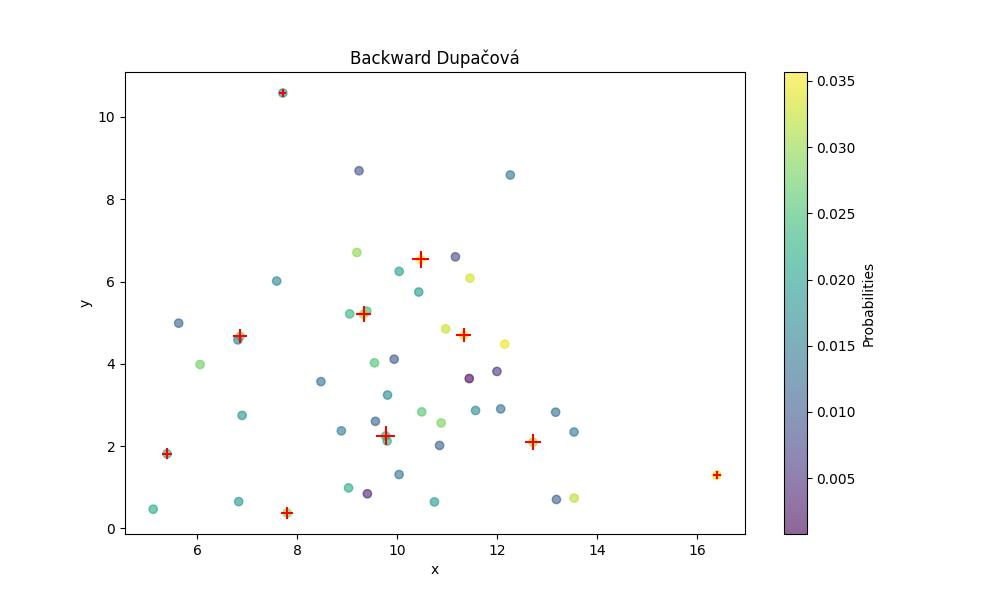
\includegraphics[width=\textwidth]{dupacova backward.jpeg}
        \caption{Output obtained with the backward algorithm}
        \label{result back}
    \end{subfigure}
    \hfill
    \begin{subfigure}[b]{0.45\textwidth}
        \centering
        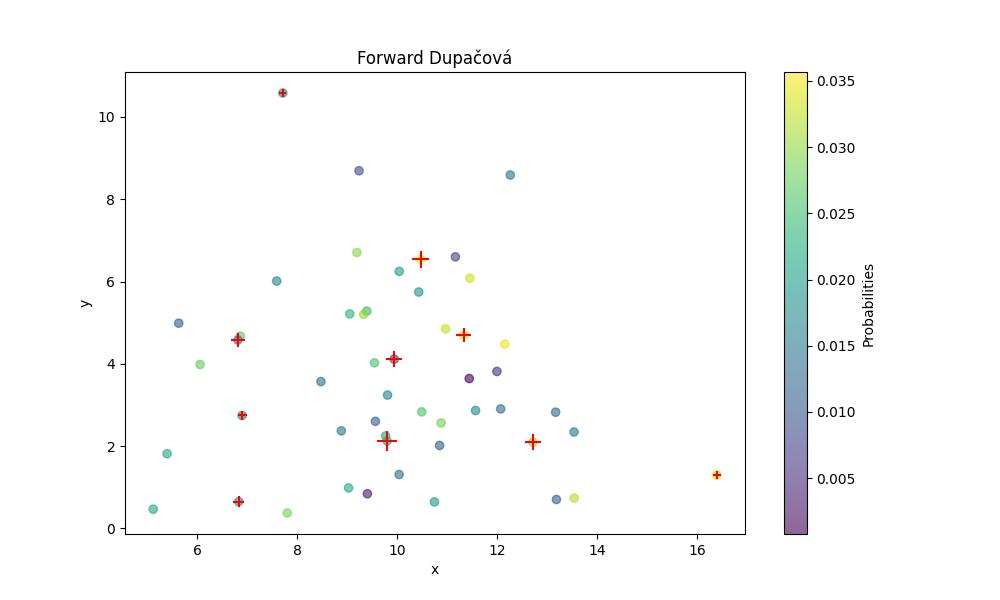
\includegraphics[width=\textwidth]{dupacova forward.jpeg}
        \caption{Output obtained with the forward algorithm}
        \label{result forw}
    \end{subfigure}
    \caption{Output visualization: forward and backward Dupačová et al' algorithm}
\end{figure}

The crosses represent atoms that are selected in the reduced set and its sizes, the amount of probability given to that point in the reduced set. As a remark, we can highlight the fact that lonely atoms are often part of the reduced set as they would impact too much the Wasserstein distance.
\subsubsection{Comparison}

\begin{figure}[ht]
    \centering
    \begin{subfigure}[b]{0.45\textwidth}
        \centering
        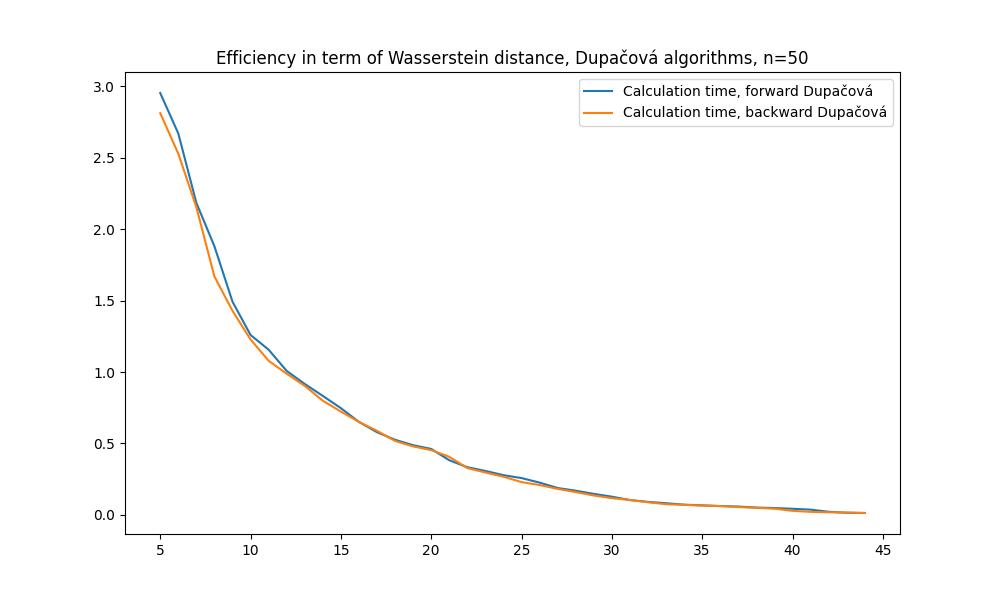
\includegraphics[width=\textwidth]{comparison forward backward distance.jpeg}
        \caption{Efficiency comparison between both algorithms}
        \label{dist for bac}
    \end{subfigure}
    \hfill
    \begin{subfigure}[b]{0.45\textwidth}
        \centering
        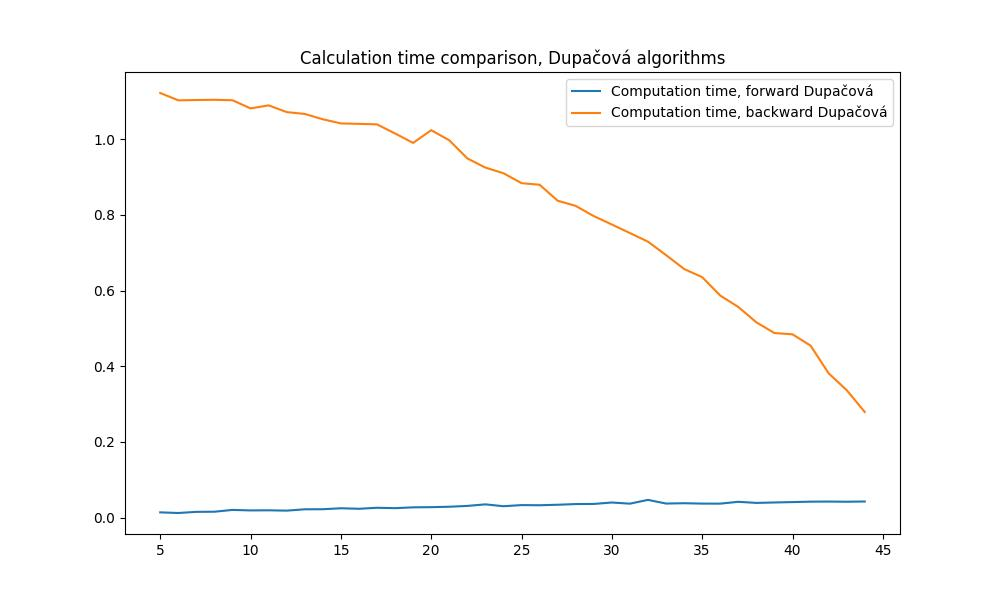
\includegraphics[width=\textwidth]{comparison forward backward time.jpeg}
        \caption{Calculation time comparison between both algorithms}
        \label{time for bac}
    \end{subfigure}
    \caption{Efficiency and calculation time comparison: forward and backward Dupačová et al' algorithm}
    \label{comparison dup}
\end{figure}

The "x" axis of \Cref{comparison dup} represents the number of atoms in the reduced set. \Cref{dist for bac} shows that the efficiency in term of Wasserstein distance is similar and comparable for a reduced set obtained via forward or backward algorithm. The main difference lies in calculation time, the efficient way to compute the forward algorithm shows its advantages in \Cref{time for bac}, always below 0.05s whereas the backward algorithm can take up to one second. Without a more efficient way than the one I proposed to compute the backward algorithm, the forward algorithm has to be preferred when you're free to choose. This data-set of 50 atoms is little compared to what you could see in real problems, the calculation time will grow as $n$ grows, that's why I make this remark. The complexity of the forward algorithm is : $\mathcal{O}\left(mn^2\right)$ whereas the backward is $\mathcal{O}\left(\left(n-m\right)^3n\right)$ with no gains of the distance. To give you an idea on what happens with a larger data-set, a 300 atoms data-set generated on the same behaviour that has to be reduced to 100 atoms: takes 4.4 seconds for the forward algorithm and 1286 for the backward. This aligns with the complexity we gave, if we define $f$ the calculation time of one operation, the order of magnitude of $f$ \rp{ordre de grandeur }is: 
\begin{align*}
mn^2f=4.4 \implies f= 4.4\times 10^{-7} \\
\left(n-m\right)^3nf=1286 \implies f=5.35\times 10^{-7}.
\end{align*}
Both $f$ have the same magnitude, it is satisfying.


\clearpage
\section{Efficient implementation}
The main goal of the internship was first to study the scenario reduction problem and algorithms related to this problem and then to implement it within the SMS++ ecosystem. SMS++ aims to deliver an efficient interface for a wide range of optimization problems through the concept of block which represents a type of problem namely "BinaryKnapsackBlock", "MCFBlock" (for Min-Cost flow) and many others. Developped in C++, it is to be able to manage memory, calculation what can be somewhat difficult in interpreted languages such as Python or Julia. In SMS++ it is easy and almost free to turn ON/OFF variables (decision variables, constraints...). In this part, we'll try to find ways to implement proficiently Dupačová et al's algorithm \Cref{dupacova} and local search algorithm \Cref{Local search}.

\subsection{Dupačová et al's algorithm}
In this part we try to reduce computational time of Dupačová et al's algorithm, meaning we want to reuse what we've already computed. 
\newline

Knowing the closed formula of \Cref{closed formula}, it isn't hard to find an efficient way to compute $D_l$ of step 2 : 
$$
D_l\left(\mathbb{P},R\cup \{y_j\}\right)=\sum_{i\in I}p_i\min_{z\in R\cup\{y\}}\lVert x_i-z \rVert^l.
$$
An efficient idea would be to store at iteration $0$, one big matrix of distance, which is : 
$$
D = \left(\lVert x_i-x_j\rVert ^l \right)_{i,j}.
$$
Then you can choose the first atom $x$ to add to R as :
$$
i_1 \in \argmin_{i\in I} pD^i.
$$
With $D^i$ being the $i^{th}$ column of $D$ and $p=\begin{pmatrix}
    p_1 & \hdots & p_n
\end{pmatrix}$.
We create $m^1=D^{i_1}$. For the second iteration, we can only select the indexes $[\![1;n]\!]\setminus \{i_1\}$. For each $x_i\in [\![1;n]\!]\setminus \{i_1\}$, let's create a vector $m_i$ such that : $\left(m_i\right)_j=\min\left\{\left(m^1\right)_j,\left(D^i\right)_j\right\}$, now we can write $D_l$ as : $$
D_l\left(\mathbb{P},\{x_{i_1}\}\cup \{x_i\}\right)=pm_i.
$$
Then follows the efficient algorithm :
\begin{algorithm}
\caption{Efficient Dupačová et al}
Initialize the set of atoms in the reduced set as $R \gets \emptyset$.\\
Compute the matrix $D = \left(\| x_i - x_j \|^l \right)_{i,j \in I^2}$ once and for all.\\
Create $m^0 = \begin{bmatrix} a & \hdots & a \end{bmatrix}$ with $a$ arbitrarily large (choose $a \geq \max_{i,j} \| x_i - x_j \|^l$).\\
\While{$|R| < m$}{
    Select the next atom to be added from $I \setminus R$ by following this procedure.\\
    \For{$i \in I \setminus R$}{
        Compute $\left(m_i\right)_j = \min \left\{ \left(m^0\right)_j, \left(D^i\right)_j \right\}$.\\
        Compute $D_l(\mathbb{P}, R \cup \{x_i\}) = p m_i$.\\
        Store the best $m_i$ so far, named $m_{\text{best}}$.\\
    }
    Update $m^0 = m_{\text{best}}$. \\
    Update $R = R \cup \{x_{\text{best}}\}$.\\
}
\Return $R$\\
\end{algorithm}

\subsection{Local search algorithm}
The same approach doesn't work for the local search as you swap atoms. An idea would have been to store an index vector, a vector that tells you with atom reaches $\min_{x\in R}\lVert x_i-x\rVert^l$ so that you know when you have to compute again the minimum on $R$ (whenever the swap removes the atom reaching the minimum). That doesn't look very efficient, but it would have looked that way : 
\begin{algorithm}
\caption{Maybe efficient local search}
Initialize the set of atoms in the reduced set $R, \lvert R\rvert=m$.\\
Compute the matrix $D = \left(\| x_i - x_j \|^l \right)_{i,j \in I^2}$ once and for all.\\
Create $m^0 = \begin{pmatrix}\min_{i\in R}\lVert x_1-x_i\rVert^l & \hdots & \min_{i\in R}\lVert x_1-x_i\rVert^l \end{pmatrix}$ and $I=\begin{pmatrix}\argmin_{i\in R}\lVert x_1-x\rVert^l & \hdots & \argmin_{i\in R}\lVert x_1-x\rVert^l \end{pmatrix}$.\\
Create $d=pm^0$, there is improvement. \\
\While{\text{ There is improvement}}{
    There isn't improvement. \\
    \For{$i \in R$}{
    Make a copy of I in index.\\
    Make a copy of $m^0$ in m. \\
        \For{$k\in I$}{
            \If{index$\left[k\right]=i$}{
                Change $\left[m\right]_k$ by $\min_{\alpha\in R\setminus\{i\}}\lVert x_k-x_\alpha\rVert^l$ and $index\left[k\right]$ aswell.
            }
        }
        \For{$j\in I\setminus R$}{
            Compute $\left(m_{ij}\right) = \min \left\{ m, D^j \}\right\}$ where $\min$ is the minimum component-wise.\\ Compute $D_l(\mathbb{P}, R \cup \{x_i\}) = p m_{ij}$.\\
            \If{$pm_{ij} < d$}{
                $d=pm_{ij}$ and there is improvement ! \\
                You can exit the \textbf{for} $i\in R$ loop if you want first-fit with , or you can keep going the for loop until you find the best-fit as $d$ is now worth $pm_{ij}$.
            }
        }
        Store the best $m_{ij}$ so far, named $m_{\text{best}}$.\\
    }
    \If{There is improvement}{
    Update $m^0 = m_{\text{best}}$. \\
    Update $R = R \cup \{x_j\} \setminus \{x_i\}$.}
}
\end{algorithm}
There is still a lot of computation here in order to compute the $\min$ inside the closed formula (we go through a vector : index, $m-1$ columns of a matrix in order to find $\min_{i\in R\setminus x_j}\lVert x_k-x_i\rVert^l$ with a complexity $\mathcal{O}\left(mn\right)$). 
%\section{Entropic regularization}
%We often need to compute $d_l\left(\mathbb{P},\mathbb{Q}\right)$ with $\mathbb{P}$ the initial distribution to be reduced and $\mathbb{Q}$ the reduced distribution in construction and solving these linear programs can be very costly as $n,m,d$ grow. 
%\begin{corollary}[Number of linear programs solved]
%    Dupačová et al's algorithm solves $$\sum_{i=0}^{m-1}n-i=m(n+\frac{1}{2})-\frac{1}{2}m^2$$ linear programs. 
%\end{corollary}
%\begin{corollary}[Number of linear programs solved]
%    The local search algorithm solves at most $$\lceil \frac{\binom{n}{m}}{\left(n-m\right)\left(m-1\right)}\rceil m\left(n-m\right)$$ linear programs when using best-first strategy.  \rp{the factor in front is in fact not true, need to think more}
%\end{corollary}
%\begin{proof}
%    Each iteration computes $m\left(n-m\right)$ linear programs so the number of linear programs solved can be written as $km\left(n-m\right)$. We have to find the largest $k$. Let $X^i$ be the vector of selected atoms at iteration $i$, what happens now is that we check the distance to $\mathbb{P}$ with all $X^i$ where you change only one atom of $X^i$ with one atom of $\text{supp}\left(\mathbb{P}\right)\setminus X^i$. If there's a closer distribution then you change the atom with the one that makes the distance smaller. So you've checked $m\left(n-m\right)$ combinations (amongst the $\binom{n}{m}$ possible, you select $m$ atoms amongst $n$ atoms without order)\rp{the factor in front is in fact not true, need to think more}
%\end{proof}
%Solving these optimal transport problems to get the value $d_l$ can be very demanding itself and it is often required. \cite[Chapter 4]{peyre_computational_2019} presents entropic regularization in the context of optimal transport. The objective function considered in the OT problem will be slightly modified by adding a convex term. Solving this new problem will be faster and it is granted that this new distance is close to the real distance of Wasserstein. 
%The regularized problem is defined as : 
%$$
%R_l^\epsilon\left(\mathbb{P},\mathbb{Q}\right)=\min_{\pi}\left\{\sum_{i\in I}\sum_{j\in J}\pi_{ij}\lVert x_i-y_j\rVert+\epsilon\sum_{i\in I}\sum_{j\in J}\pi_{ij}\left(\log{\left(\pi_{ij}\right)}-1\right)\right\}
%$$


\clearpage
\appendix
\section{Wasserstein distance is a distance}\label{distance}
In this appendix, we prove that Wasserstein distance is indeed a distance whenever $l\geq1$.
\begin{enumerate}
    \item $d_l$ has values in $\RR_+$.
    \item Symmetry is easy.
    \item Definiteness requires a little more work. First, we prove that $d_l\left(\mathbb{P},\mathbb{Q}\right)=0\implies \text{supp}\left(\mathbb{P}\right)=\text{supp}\left(\mathbb{Q}\right)$. Alright, let $\mathbb{P}=\sum_{i\in I}\delta_{x_i}p_i,\mathbb{Q}=\sum_{j\in J}\delta_{y_j}q_j$ such that $d_l\left(\mathbb{P},\mathbb{Q}\right)=0$, let's assume that $\text{supp}\left(\mathbb{P}\right)\ne\text{supp}\left(\mathbb{Q}\right)$. Then there exists $x_{i_0}\in \text{supp}\left(P\right)$ such that $x_{i_0}\neq y, \:\forall y\in\text{supp}\left(\mathbb{Q}\right)$ (if not, then a $y_{i_0}$ exists in $\text{supp}\left(Q\right)$ and $y_{i_0}\notin \text{supp}\left(P\right)$ as the support are different but it's the same, it doesn't matter). As $d_l\left(\mathbb{P},\mathbb{Q}\right)=0$ we have that :$$
    \exists\pi\in\RR^{nm}_+ : \sum_{i\in I}\pi_{ij}=q_j, \sum_{j\in J}\pi_{ij}=p_i, \forall i,j \text{ and } \sum_{j\in J}\sum_{i\in I}\pi_{ij}\lVert x_i-y_j\rVert^l=0.
    $$
    Look at the last equation, each term of the sum is positive, then it follows that :
    \begin{equation}\label{useful}
    \forall i,j \in I\times J, \: \pi_{ij}\lVert x_i-y_j\rVert^l=0.
    \end{equation}
    and you can forget the $l^{th}$ power without a single remorse :
    $$
     \forall i,j \in I\times J, \: \pi_{ij}\lVert x_i-y_j\rVert=0.
    $$
    But we said that there exists $x_{i_0}\in\text{supp}\left(P\right)\setminus\text{supp}\left(Q\right)$. It follows that $\forall j\in J, \pi_{i_0j}=0$ what's impossible because of the constraints we had, $0=\sum_{j\in J}\pi_{i_0j}=p_{i_0}\neq0.$ First step : check ! $$d_l\left(\mathbb{P},\mathbb{Q}\right)=0\implies \text{supp}\left(\mathbb{P}\right)=\text{supp}\left(\mathbb{Q}\right).$$
    W.l.o.g. we can renumber the atom and then say $p_i$ and $q_i$ are associated to the same atom. We use \Cref{useful} and we have that :
    $$
    \forall k\in I, k\neq i, \pi_{ki}=0, \pi_{ik}=0.
    $$
    Then the constraints on $\pi$'s sum on rows and columns give  : $$ 
    \sum_{k\in I}\pi_{ki}=\pi_{ii}=q_i \text{ and } \sum_{k\in J}\pi_{ik}=\pi_{ii}=p_i.
    $$
    We've proven the definiteness of $d_l$. Because supports and weights are the same for both distribution : $\mathbb{P}=\mathbb{Q}$.
    \item Triangle inequality, see \cite[Proposition 2.2]{peyre_computational_2019}
\end{enumerate}
\begin{remark}
    If $0<l<1, d_l^l$ is a distance.
\end{remark}
\section{Computing Wasserstein distance}
\label{compute}
Let $\mathbb{P}=\sum_{i\in I}\delta_{x_i}p_i, \mathbb{Q}=\sum_{j\in J}\delta_{y_j}q_j$ two finite distributions. Computing the distance is equivalent to solving a linear program. Thus it is "easily" computable (with the simplex or with better-fitting techniques as it is a min-cost transportation problem).
If we write $n=|I|, m=|J|$ and :
$$
\pi=\begin{bmatrix}
    \pi_{11}& \hdots&\pi_{1m}&\pi_{21}&\hdots&\pi_{2m}&\hdots\pi_{nm}
\end{bmatrix}^T.
$$
Than the constraints can be visualized with the matrix $A=\begin{pmatrix}
    A_I \\
    A_J
\end{pmatrix}$ with $A_I$ $k^{th}$ row (out of the $n$ rows) being : 
$$\begin{bmatrix}
    0&\hdots&0&1&\hdots&1&0&\hdots&0
\end{bmatrix}.$$
with $m\times(k-1)$ zeros at the beginning, then $m$ ones and then zeros. 
\newline
Similarly $A_J$ $k^{th}$ row (out of the $m$ rows) is full of zeros except at position $k+(j-1)\times m, \forall j\in J$ where you'll find ones. This way, it's easy to find a distance between two finite distributions.
\newline

One more thing we can say is that $rk(A)=n+m-1$. The rows of A are linearly dependant : $L_1+...+L_n-L_{n+1}-...-L_{n+m}=0$. Then if we take a linear combination of rows $A_1,...,A_{n+m-1}$ that is equal to zero, we have that $$
\sum_{i=1}^{n+m-1}\lambda_iL_i^T=\begin{bmatrix}
    \lambda_1+\lambda_{n+1}\\ \vdots\\ \lambda_1+\lambda_{n+m-1}\\ \lambda_{1} \\ \lambda_2+\lambda_{n+1} \\ \vdots \\ \lambda_2+\lambda_{n+m-1}\\ \lambda_2  \\ \vdots
\end{bmatrix}=0_{\RR^{nm}}.
$$
Directly, we see that $\forall i \in [\![1;n]\!], \lambda_i=0$ when we look at the $(m\times i)^{th}$ coefficient and then $\forall k\in[\![1;n+m-1]\!], \lambda_k=0$ is easy to see. Then $rk(A)=n+m-1$. \rp{kind of useless as we know that the number of variables in basis is $n+m$ (number of constraints) but can be the starting point of sparsity explanation if I study regularization as Benoît mentionned}
\section{Scaled distribution and Wasserstein distance}
\label{scaled}
 Let $m\in\mathbb{N}^*$, $\mathbb{Q}\in\mathcal{P}(X,m) $ and $\lambda\in\RR^*$. We have that
\begin{align*}
    d_l(\mathbb{P}^\lambda,\mathbb{Q})^l&=\min_{\pi\in\mathbb{R_+^{|I|\times|J|}}}\left\{ 
\sum_{i\in I}\sum_{j\in J}\pi_{ij}\lVert\lambda x_i-y_j\rVert^l \: \text{ : } \:  \begin{aligned}
& \sum_{j\in J}\pi_{ij}=p_i \: \forall i\in I \\
& \sum_{i\in I}\pi_{ij}=q_j \: \forall j\in J
\end{aligned}\right\} \\&=\lambda^l\cdot\min_{\pi\in\mathbb{R_+^{|I|\times|J|}}}\left\{ 
\sum_{i\in I}\sum_{j\in J}\pi_{ij}\lVert x_i-\frac{1}{\lambda}y_j\rVert^l \: \text{ : } \:  \begin{aligned}
& \sum_{j\in J}\pi_{ij}=p_i \: \forall i\in I \\
& \sum_{i\in I}\pi_{ij}=q_j \: \forall j\in J
\end{aligned}\right\} \\
&=\lambda^l \cdot d_l(\mathbb{P},\mathbb{Q}^{\frac{1}{\lambda}})^l.
\end{align*}
Taking the $\frac{1}{\lambda}^{th}$ power gives :  $d_l(\mathbb{P}^\lambda,\mathbb{Q})=\lambda\cdot d_l(\mathbb{P},\mathbb{Q}^{\frac{1}{\lambda}})$. Now, we have $$C_l(\mathbb{P}^\lambda,m)\leq d_l(\mathbb{P}^\lambda,\mathbb{Q})=\lambda\cdot d_l(\mathbb{P},\mathbb{Q}^{\frac{1}{\lambda}})$$
But the left hand side doesn't depend on $\mathbb{Q}$ any longer so we can minimize the right hand side over $\mathbb{Q}\in\mathcal{P}(X,m)$ almost directly $C_l(\mathbb{P},m)=\min_\mathbb{Q}\left\{d_l(\mathbb{P},\mathbb{Q}),\: \mathbb{Q}\in\mathcal{P}(\mathbb{R}^d,m)\right\}=\min_\mathbb{Q}\left\{d_l(\mathbb{P},\mathbb{Q}^\frac{1}{\lambda}),\: \mathbb{Q}\in\mathcal{P}(\mathbb{R}^d,m)\right\}$ :
$$
C_l(\mathbb{P}^\lambda,m)\leq \lambda\cdot C_l(\mathbb{P},m).
$$
Similarly we can prove : $C_l(\mathbb{P}^\lambda,m)\geq \lambda\cdot C_l(\mathbb{P},m)$, both results prove the positive homogeneity of the Wasserstein distance.
The result holds for $\lambda=0$. $m\geq 1$ (don't you dare trying to reduce a distribution to a distribution without a single atom...), $\mathbb{P}^0=\delta_0$. We have that : $$0\leq C_l(\mathbb{P}^0,m)\leq d_l(\mathbb{P}^0,\delta_0)=0.$$
\section{Scaled distribution and Wasserstein distance 2.0}
\label{scaled 2}
Using what we did in the appendix above, with $\mathbb{Q}\in\mathcal{P}\left(\text{supp}\left(P\right),m\right)\subset \mathcal{P}(X,m)$, it's easy to verify that $\mathbb{Q}^\lambda\in\mathcal{P}\left(\text{supp}\left(P^\lambda\right),m\right)$ and we have that : $$\lambda D_l\left(\mathbb{P},m\right)\leq \lambda d_l\left(\mathbb{P},\mathbb{Q}\right)=d_l\left(\mathbb{P}^\lambda,\mathbb{Q}^\lambda\right).$$ 
Similarly to the above appendix, we can now minimize the right hand side because the left hand side doesn't depend on $\mathbb{Q}, \lambda$.
We have :
$$
\lambda D_l\left(\mathbb{P},m\right)\leq D_l\left(\mathbb{P}^\lambda,m\right).
$$
The exact same thing works in order to get : 
$$
\lambda D_l\left(\mathbb{P},m\right)\geq D_l\left(\mathbb{P}^\lambda,m\right).
$$
Meaning that : 
$$
\lambda D_l\left(\mathbb{P},m\right)=D_l\left(\mathbb{P}^\lambda,m\right).
$$
As a reminder, we've proven the same thing for $C_l$. Works too when $\lambda= 0$.
\section{Re-positionning and Wasserstein distance}
We want to prove that re-positionning doesn't affect $C_l$ ($D_l$ equally). Let $\mathbb{P}=\sum_{i\in I}\delta_{x_i}p_i,\mathbb{Q}=\sum_{j\in J}\delta_{y_j}q_j, a\in\RR^d$. Let's write : $\mathbb{P}_a=\sum_{i\in I}\delta_{x_i+a}p_i$. 
\begin{align*}
d_l(\mathbb{P}_a,\mathbb{Q})&=\left(\min_{\pi\in\mathbb{R_+^{|I|\times|J|}}}\left\{ 
\sum_{i\in I}\sum_{j\in J}\pi_{ij}\lVert (x_i+a)-y_j\rVert^l \: \text{ : } \:  \begin{aligned}
& \sum_{j\in J}\pi_{ij}=p_i \: \forall i\in I \\
& \sum_{i\in I}\pi_{ij}=q_j \: \forall j\in J
\end{aligned}\right\}\right)^{1/l}
\\ &= \left(\min_{\pi\in\mathbb{R_+^{|I|\times|J|}}}\left\{ 
\sum_{i\in I}\sum_{j\in J}\pi_{ij}\lVert x_i-(y_j-a)\rVert \: \text{ : } \:  \begin{aligned}
& \sum_{j\in J}\pi_{ij}=p_i \: \forall i\in I \\
& \sum_{i\in I}\pi_{ij}=q_j \: \forall j\in J
\end{aligned}\right\}\right)^{1/l}
\\ &=d_l\left(\mathbb{P},\mathbb{Q}_{-a}\right)
\end{align*}
Let's do it again... alright. Let $\mathbb{Q}\in\mathcal{P}\left(\RR^d,m\right)$, we have that :
$$
C_l\left(P_a,m\right)\leq d_l\left(\mathbb{P}_a,\mathbb{Q}\right)=d_l\left(\mathbb{P},\mathbb{Q}_{-a}\right).
$$
Once again, yes, the left hand side doesn't depend on $\mathbb{Q}, a$ and $\mathbb{Q}_{-a}\in\mathcal{P}\left(\RR^d,m\right)$, it follows that :
$$
C_l\left(P_a,m\right)\leq C_l\left(P,m\right).
$$
And we can do the same thing to get the opposite inequality, then we have : 
$$
C_l\left(P_a,m\right)= C_l\left(P,m\right).
$$
\section{Eigenvalues of a matrix invariant under permutations}
 \label{eigen}
 A matrix $A$ that is invariant under permutations can be written as $A=\alpha I_n + \beta \mathbf{1}\mathbf{1}^T$ whose characteristic polynomial is :
$$\chi_A(X)=\text{det}(\begin{bmatrix}
    X- \alpha - \beta & -\beta&\hdots&-\beta \\
    -\beta & \ddots &\ddots&\vdots \\
    \vdots &\ddots &\ddots&   \\
    &&&-\beta\\
    -\beta&\hdots&-\beta&X-\alpha-\beta
\end{bmatrix})=(X-\alpha-n\beta)\text{P}_{A_1}\left(X\right).$$
where $\text{P}_{A_1}\left(X\right)$ is the determinant of the matrix $XI_n-A$ with its first column replaced by a column of ones. The first equality arises from adding every column to the first one, so the first column is a column of $X-\alpha-n\beta$, so we can factorize by $X-\alpha-n\beta$. What we have to do next is do add $\beta\cdot C_1$ ($C_1$ is the column of ones) to every other column, what gives us a lower triangular matrix with the diagonal $diag(1,X-\alpha,...,X-\alpha)$, and we have $$
\chi_A(X)=(X-\alpha-n\beta)(X-\alpha)^{n-1}$$

\section{Chebyshev center problem for the norm L2}
\label{chebyshev}
The Chebyshev problem is :
\begin{align*}
    &\min_{r,\mu} \quad r\\
    &\text{s.t.}\quad \lVert x_i-\mu\rVert^2-r^2 \leq 0, \;\forall i\in I.\\
    &-r\leq0
\end{align*}
We can write the Lagrangian of this problem : 
$$
\mathcal{L}(r,\mu,\lambda)=r+\lambda_0r+\sum_{i\in I}\lambda_i(\lVert x_i-\mu\rVert^2-r^2)
$$
KKT conditions provide at optimality : \begin{align*}
    \lambda\geq0\\
    \nabla_r\mathcal{L}(r,\mu,\lambda)=0\\
    \nabla_\mu\mathcal{L}(r,\mu,\lambda)=0\\
    \forall i\in I,\;\lambda_i(\lVert x_i-\mu\rVert^2-r^2)=0 \\
    \lambda_0r=0
\end{align*}
The gradient isn't always defined according to the norm but when it's $\lVert\cdot\rVert_2$ : 
\begin{align*}
    \lambda\geq0\\
    1+\lambda_0-2r\sum_{i\in I}\lambda_i=0\\
    \sum_{i\in I}\lambda_i(x_i-\mu)=0\\
    \forall i\in I,\;\lambda_i(\lVert x_i-\mu\rVert^2-r^2)=0 \\
    \lambda_0r=0
\end{align*}
All $\lambda_i, \: i\in I$ can't be $0$, otherwise, the equation $1+\lambda_0-2r\sum_{i\in I}\lambda_i=0$ is impossible (as $\lambda_0$ is also positive). Then, there exists $i\in I$ such that $\lambda_i>0$, for this particular $i$, $\lVert x_i-\mu\lVert^2=r^2$. Moreover, initial constraints give that :
$$
r^2\geq \max_{i\in I}\lVert x_i-\mu \rVert^2
$$
Then we can conclude that :
$$
r^*\left(\mu\right)=\max_{i\in I}\lVert x_i-\mu\rVert^2.
$$
But we haven't found the optimal $\mu$, thus the problem becomes : 
$$
\min_{\mu\in\RR^d}r^*\left(\mu\right)=\min_{\mu\in\RR^d}\max_{i\in I}\lVert x_i-\mu\rVert^2=\min_{\mu\in\RR^d}\left\{\mu^T\mu+\max_{i\in I}\left[x_i^Tx_i-2\mu^Tx_i\right]\right\}.
$$
\section{Upgrading local search}\label{L_p optim}
In order to improve the Wasserstein distance given by local search algorithm, one must solve $m$ times: 
$$
\min_{y\in\RR^d}\sum_{i\in I}p_i\lVert x_i-y\rVert^\ell=\min_{y\in\RR^d}\sum_{i\in I}p_i\left(\lVert x_i-y\rVert^2\right)^{\ell/2}.
$$
With $p_i>0$, $I$ a particular set and for an arbitrary norm, in most cases we'll use $\text{L}2$-norm. For this particular norm, the case $\ell=1$ gives the geometric median and $\ell=2$ gives the mean. With L$2$-norm, the function $f$ to minimize is differentiable and we can write : 
$$
\nabla f\left(y\right)=-\ell\sum_{i\in I}p_i\lVert x_i-y\rVert^{\ell-2}\left(x_i-y\right).
$$
Any gradient-based method would be efficient to solve this problem. \rp{can be interesting to study more but hard to find references}
\bibliography{biblio}
\bibliographystyle{alpha}
\end{document}
